% Template for Cogsci submission with R Markdown

% Stuff changed from original Markdown PLOS Template
\documentclass[10pt, letterpaper]{article}

\usepackage{cogsci}
\usepackage{pslatex}
\usepackage{float}
\usepackage{caption}

% amsmath package, useful for mathematical formulas
\usepackage{amsmath}

% amssymb package, useful for mathematical symbols
\usepackage{amssymb}

% hyperref package, useful for hyperlinks
\usepackage{hyperref}

% graphicx package, useful for including eps and pdf graphics
% include graphics with the command \includegraphics
\usepackage{graphicx}

% Sweave(-like)
\usepackage{fancyvrb}
\DefineVerbatimEnvironment{Sinput}{Verbatim}{fontshape=sl}
\DefineVerbatimEnvironment{Soutput}{Verbatim}{}
\DefineVerbatimEnvironment{Scode}{Verbatim}{fontshape=sl}
\newenvironment{Schunk}{}{}
\DefineVerbatimEnvironment{Code}{Verbatim}{}
\DefineVerbatimEnvironment{CodeInput}{Verbatim}{fontshape=sl}
\DefineVerbatimEnvironment{CodeOutput}{Verbatim}{}
\newenvironment{CodeChunk}{}{}

% cite package, to clean up citations in the main text. Do not remove.
\usepackage{apacite}

% KM added 1/4/18 to allow control of blind submission


\usepackage{color}

% Use doublespacing - comment out for single spacing
%\usepackage{setspace}
%\doublespacing


% % Text layout
% \topmargin 0.0cm
% \oddsidemargin 0.5cm
% \evensidemargin 0.5cm
% \textwidth 16cm
% \textheight 21cm

\title{Integration of gaze information in online language comprehension and
learning}

\usepackage{threeparttable}
\usepackage{booktabs}

\author{{\large \bf Kyle MacDonald (kemacdonald@ucla.edu)} \\ Department of Communication, UCLA  \AND {\large \bf Elizabeth Swanson (elizswan@stanford.edu)} \\ Department of Psychology, Stanford University  \AND {\large \bf Michael C. Frank (mcfrank@stanford.edu)} \\ Department of Psychology, Stanford University  }

\begin{document}

\maketitle

\begin{abstract}
Face-to-face communication provides listeners with access to visual
information that can support language processing. But do listeners
automatically seek social information without regard to the learning
problem? Here, we present two eye-tracking studies that ask whether
listeners' knowledge of word-object links changes how they actively
gather an ecologically-valid social cue to reference (a speaker's eye
gaze) during real-time language processing. First, when processing
highly familiar words, children and adults did not delay their gaze
shifts to seek a fully disambiguating gaze cue. When processing novel
words, however, children and adults fixated longer on a speaker who
provided a gaze cue, which, in turn, led to an increase in looking to
the named object and less looking to the other object in the scene.
These results suggest that learners integrate their knowledge of object
labels when deciding how to allocate visual attention to social
partners, which in turn could shape the input to word learning
mechanisms.

\textbf{Keywords:}
eye movements; language processing; information-seeking; word learning;
gaze following
\end{abstract}

\hypertarget{introduction}{%
\section{Introduction}\label{introduction}}

Understanding language is challenging. Consider that even in grounded
language comprehension, people can talk about many things, with no
guarantee that they use familiar words. This flexibility creates the
potential for a speaker's intended meaning to be largely unconstrained.
Listeners, however, can overcome ambiguity by integrating visual
information available in face-to-face communication (e.g., the direction
of a speaker's gaze) that constrains the interpretation of an utterance
(Vigliocco, Perniss, \& Vinson, 2014). But do listeners strategically
seek supportive visual information from other speakers? And does this
information seeking depend on the listener's knowledge of the incoming
language?

Prior empirical and theoretical work on language processing, shows that
listeners integrate input from multiple sources to constrain the set of
possible interpretations of an utterance (see McClelland, Mirman, and
Holt, 2006, for a review). For example, adults are faster to process
information and make fewer comprehension errors if a speaker provides
gestures with redundant cues to meaning (Kelly, Özyürek, \& Maris,
2010). Moreover, developmental research shows that parents actively use
visual cues such as gestures and direction of their gaze to structure
language interactions with their children (Estigarribia \& Clark, 2007).
And even 16-month-olds are able to use the direction of another
speaker's gaze to infer the meaning of a new word (Baldwin, 1993).

These findings suggest that visual information can facilitate language
processing. The visual signal, however, is transient and the value of
fixating on a communicative partner can vary depending on the language
processing task. Thus, rather than randomly fixate a scene, listeners
might strategically deploy their fixations to informative locations that
maximize successful comprehension. For example, in prior work, we found
that children and adults fixated longer on a speaker's face when
processing familiar words in a ``noisy'' auditory environment,
suggesting that they compensated for uncertainty in the auditory signal
by gathering more visual information (MacDonald, Marchman, Fernald, \&
Frank, 2018). Moreover, recent theoretical and empirical work suggests
that children and adults handle noise in the signal by integrating what
they perceive with their prior beliefs about the speaker's intended
meaning (Fourtassi \& Frank, 2017; Gibson, Bergen, \& Piantadosi, 2013;
Yurovsky, Case, \& Frank, 2017).

Here, we pursue the idea that the value of fixating on another speaker
could vary as a function of (1) the helpfulness of the interlocutor and
(2) the listeners' prior experience with a word-object link. In two
experiments, we manipulate whether a speaker provides a valid visual cue
to reference: by directing her eye gaze to an object while either
producing a concrete, familiar word (``ball'', E1) or a novel word
(``dax'', E2). We chose this behavior as a case study of active
information seeking because gaze following is thought to be relevant for
the ecological task of linking language to the world and recent work has
found a reliable link between sustained visual attention on objects and
word learning (Smith \& Yu, 2013).

Our second goal is to test whether children and adults would show a
similar pattern of adapting the timing of their gaze shifts to gather a
social cue to reference. It could be that children rely more on visual
information from social partners because they have partial knowledge of
word-object links and are developing a language model. Moreover, adults
have more prior experience with the familiar words in our study and
stronger novel word learning skills. Both of these features could
diminish the usefulness of seeking a social cue when they process
familiar or novel words.

\begin{CodeChunk}
\begin{figure*}[h]

{\centering 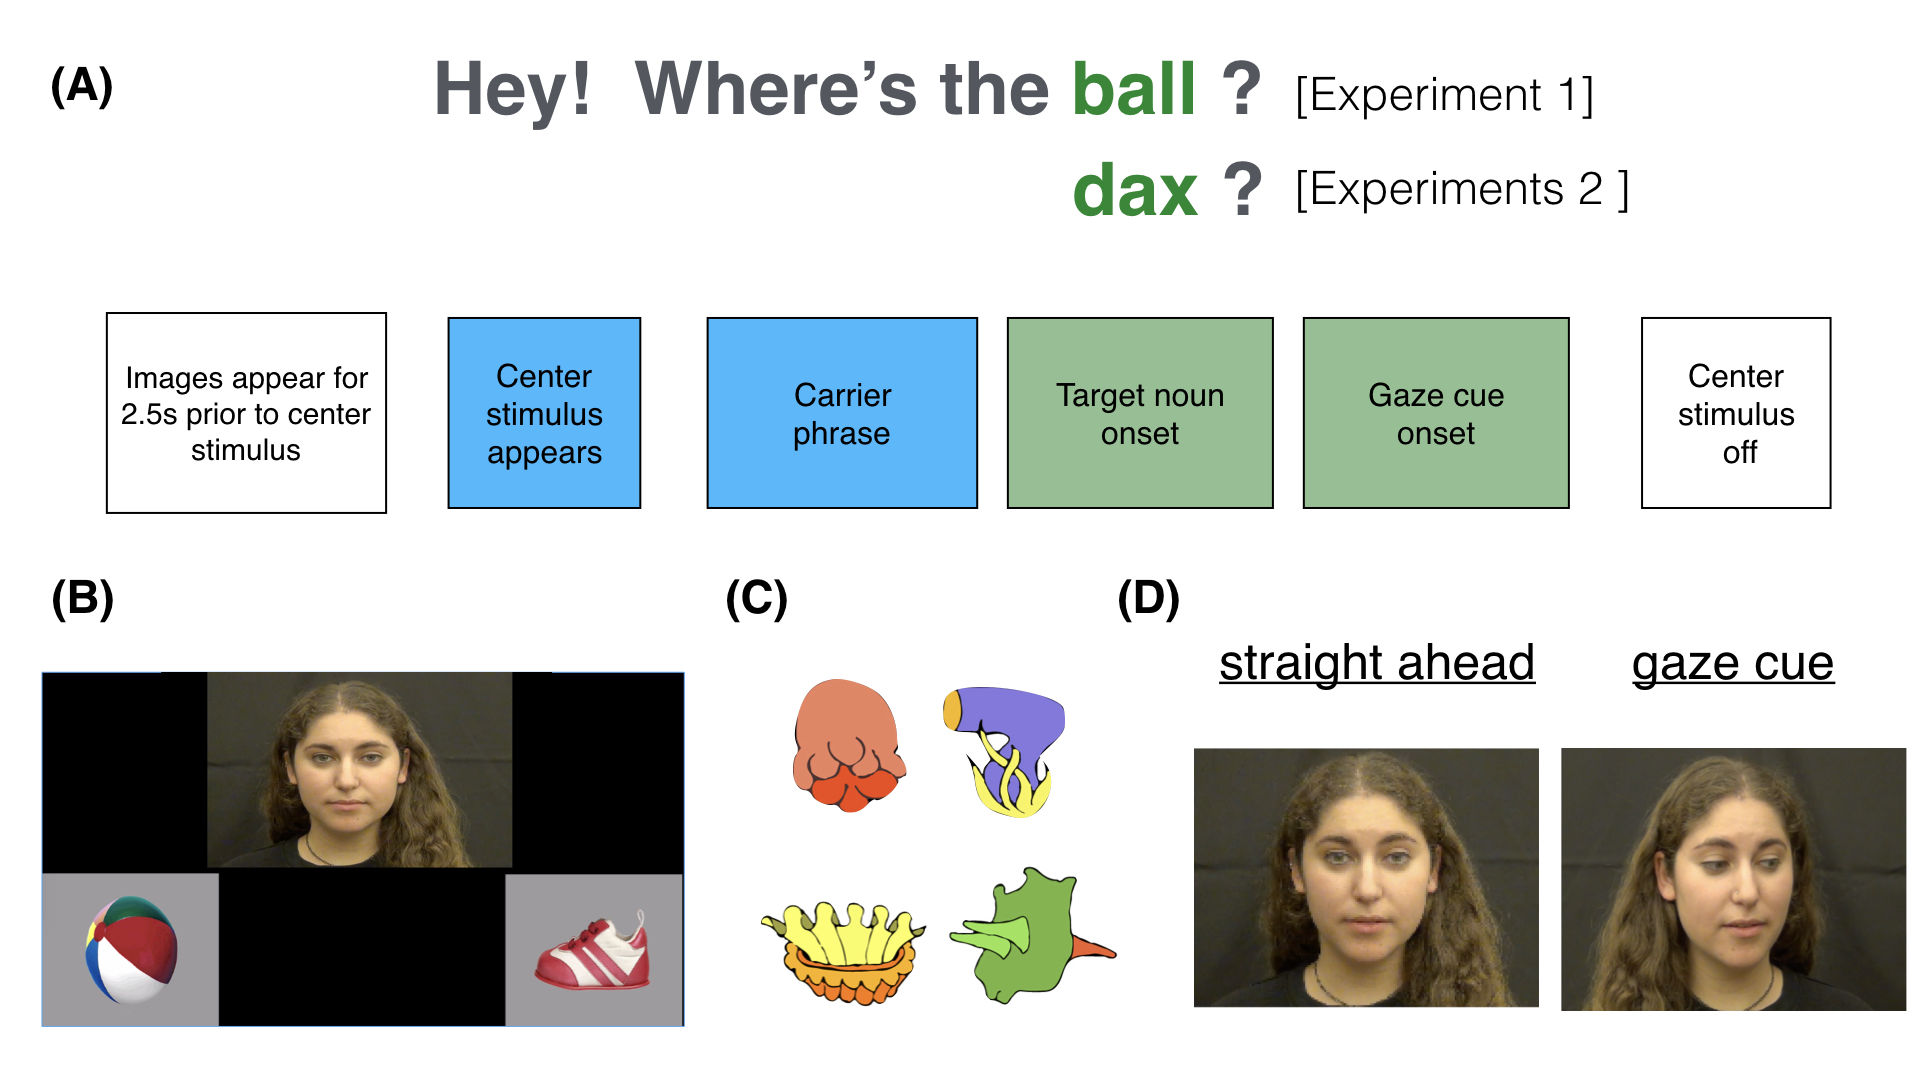
\includegraphics[width=0.65\linewidth]{/Users/kylemacdonald/Documents/Projects/SPEED-ACC-NOVEL/writing/figures/plots/gaze_stimuli} 

}

\caption[Stimuli for Experiments 1 and 2]{Stimuli for Experiments 1 and 2. Panel A shows the structure of the linguistic stimuli for a single trial. Panel B shows the layout of the fixation locations for all tasks: the center stimulus, the target, and the distracter. Panel C shows a sample of the images used as novel objects in Experiment 2. Panel D shows an example of the social gaze manipulation.}\label{fig:gaze-stimuli}
\end{figure*}
\end{CodeChunk}

Here, we characterize eye movements as a series of information seeking
decisions that aim to minimize uncertainty about the external world
(Hayhoe \& Ballard, 2005). Under this account, listeners should consider
the utility of fixating on a speaker for achieving their current task
goal. We hypothesized that when a communicative partner produces a gaze
cue, they become more valuable for the task of disambiguating reference.
Our key behavioral prediction is that listeners will delay generating an
eye movement away from a speaker's face until seeing where she directs
her gaze. This delay will lead to an increase in fixations to the named
object.

\hypertarget{experiment-1}{%
\section{Experiment 1}\label{experiment-1}}

In Experiment 1, we measured the time course of children and adults'
decisions about visual fixation as they processed sentences with
familiar words (``Where's the ball?''). We manipulated whether the
speaker produced a post-nominal gaze cue to the named object. The visual
world consisted of three fixation targets (a center video of a person
speaking and a target/distracter picture). The primary question of
interest was whether listeners would delay shifting their gaze away from
the speaker's face if she was likely to generate a gaze cue. We
predicted that fixating longer on the speaker would allow listeners to
gather more language-relevant visual information to facilitate
comprehension. In contrast, if listeners show parallel gaze dynamics
across conditions, this would suggest that hearing the familiar word was
the primary factor driving shifts in visual attention.

\begin{CodeChunk}
\begin{figure*}[t]

{\centering 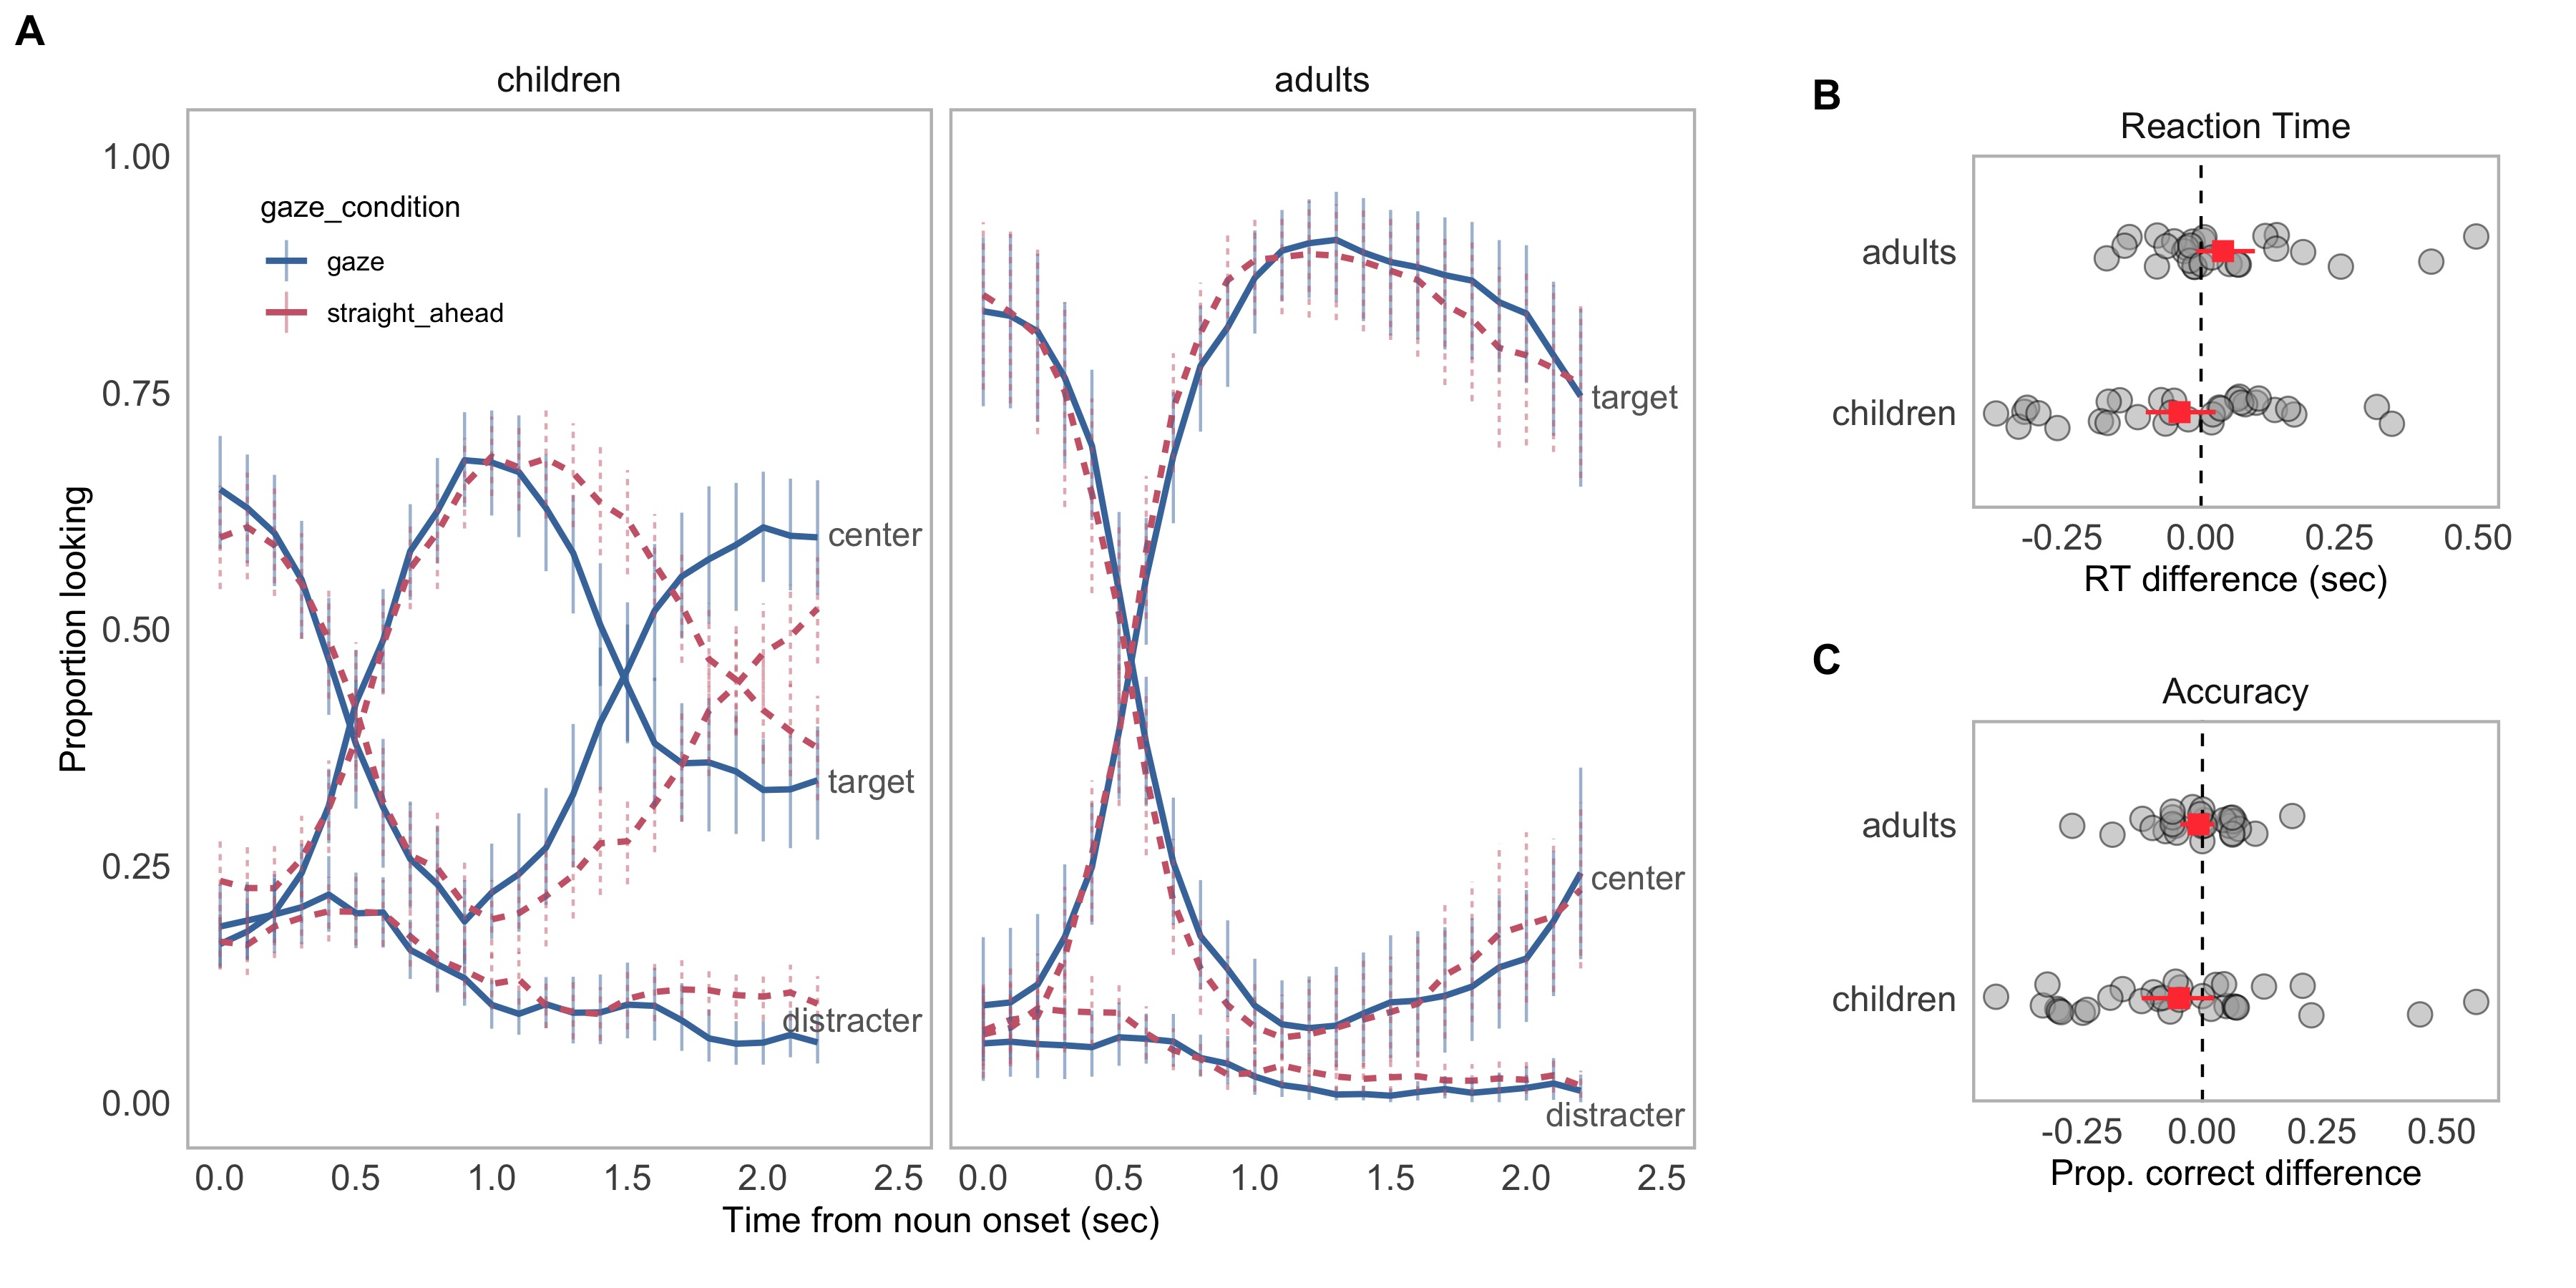
\includegraphics[width=0.9\linewidth]{/Users/kylemacdonald/Documents/Projects/SPEED-ACC-NOVEL/writing/figures/plots/speed_acc_fam_behav} 

}

\caption[Timecourse looking, first shift Reaction Time (RT), and Accuracy results for children and adults in Experiment 1]{Timecourse looking, first shift Reaction Time (RT), and Accuracy results for children and adults in Experiment 1. Panel A shows the overall looking to the center, target, and distracter stimulus for each gaze condition and age group. Panel B shows the distribution of pairwise contrasts between each participant's RT in the gaze and no-gaze conditions. The square point represents the group means. The vertical dashed line represents the null model of zero condition difference. Error bars represent the 95\% HDI. Panel C shows the same information but for first shift accuracy.}\label{fig:speed-acc-gaze-results}
\end{figure*}
\end{CodeChunk}

\hypertarget{analytic-approach}{%
\subsection{Analytic approach}\label{analytic-approach}}

To quantify evidence for our predictions, we present two analyses.
First, we analyze the time course of listeners' looking to each area of
interest (AOI). Proportion looking reflects the mean proportion of
trials on which participants fixated on the speaker, the target image,
or the distracter image at every 33-ms interval of the stimulus
sentence. We tested condition differences in the proportion looking to
the language source -- signer or speaker -- using a nonparametric
cluster-based permutation analysis, which accounts for the issue of
taking multiple comparisons across many time bins in the timecourse
(Maris \& Oostenveld, 2007). A higher proportion of looking to the
language source in the gaze condition would indicate listeners'
prioritization of seeking visual information from the speaker.

Next, we analyzed the RT and Accuracy of participants' initial gaze
shifts away from the speaker to objects in the scene. RT corresponds to
the latency of shifting gaze away from the central stimulus to either
object measured from the onset of the target noun. All reaction time
distributions were trimmed to between zero and two seconds, and RTs were
modeled in log space. Accuracy corresponds to whether participants'
first gaze shift landed on the target or the distracter object. If
listeners generate slower but more accurate gaze shifts, this provides
evidence that gathering more visual information from the speaker led to
more robust language processing in the gaze context.

We used the \texttt{brms} (Bürkner, 2017) package to fit Bayesian
mixed-effects regression models. The mixed-effects approach allowed us
to model the nested structure of our data -- multiple trials for each
participant and item, and the within-participants manipulation. We used
Bayesian estimation to quantify uncertainty in our point estimates,
which we communicate using a 95\% Highest Density Interval (HDI),
providing a range of credible values given the data and model.

\hypertarget{methods}{%
\subsection{Methods}\label{methods}}

\hypertarget{participants}{%
\subsubsection{Participants}\label{participants}}

\begin{table}[tbp]
\begin{center}
\begin{threeparttable}
\caption{\label{tab:make-ss-table}Age distributions of children in Experiments 1 and 2. All ages are reported in months.}
\begin{tabular}{lllll}
\toprule
Experiment & \multicolumn{1}{c}{n} & \multicolumn{1}{c}{Mean} & \multicolumn{1}{c}{Min} & \multicolumn{1}{c}{Max}\\
\midrule
Exp. 1 (familiar words) & 38 & 55.50 & 35.60 & 71.04\\
Exp. 2 (novel words) & 54 & 52.60 & 36.26 & 70.94\\
\bottomrule
\end{tabular}
\end{threeparttable}
\end{center}
\end{table}

Participants were native, monolingual English-learning children (\(n=\)
38; 19 F) and adults (\(n=\) 33; 23 F). All participants had no reported
history of developmental or language delay and normal vision. 12
participants (9 children, 3 adults) were run but not included because
either the eye tracker failed to calibrate (8 children, 2 adults) or the
participant did not complete the task (1 children, 1 adults).

\hypertarget{materials}{%
\subsubsection{Materials}\label{materials}}

\emph{Linguistic stimuli.} The video/audio stimuli were recorded in a
sound-proof room and featured two female speakers who used natural
child-directed speech and said one of two phrases: ``Hey! Can you find
the (target word)'' or "Look! Where's the (target word). The target
words were: ball, bunny, boat, bottle, cookie, juice, chicken, and shoe.
The target words varied in length (shortest = 412 ms, longest = 780 ms)
with an average length of 587 ms.

\emph{Gaze manipulation}. To create the stimuli in the gaze condition,
the speaker waited until she finished producing the target sentence and
then turned her head to gaze at the bottom corner of the camera frame.
After looking at the named object, she then returned her gaze to the
center of the frame. We chose to allow the length of the gaze cue to
vary to keep the stimuli naturalistic. The average length of gaze was
2.12 seconds with a range from 1.78 to 3.07 seconds.

\emph{Visual stimuli.} The image set consisted of colorful digitized
pictures of objects presented in fixed pairs with no phonological
overlap between the target and the distracter image (cookie-bottle,
boat-juice, bunny-chicken, shoe-ball). The side of the target picture
was counterbalanced across trials.

\hypertarget{procedure}{%
\subsubsection{Procedure}\label{procedure}}

Participants viewed the task on a screen while their gaze was tracked
using an SMI RED corneal-reflection eye-tracker mounted on an LCD
monitor, sampling at 30 Hz. The eye-tracker was first calibrated for
each participant using a 6-point calibration. On each trial,
participants saw two images of familiar objects on the screen for two
seconds before the center stimulus appeared. Next, they processed the
target sentence followed by two seconds without language to allow for a
response. Both children and adults saw 32 trials (16 gaze trials; 16
no-gaze trials) with several filler trials interspersed to maintain
interest. The gaze manipulation was presented in a blocked design with
the order of block counterbalanced across participants.

\hypertarget{results-and-discussion}{%
\subsection{Results and Discussion}\label{results-and-discussion}}

\hypertarget{timecourse-looking}{%
\subsubsection{Timecourse looking}\label{timecourse-looking}}

We first analyzed how the presence of gaze influenced listeners'
distribution of attention across the three fixation locations. At
target-noun onset, listeners tended to look more at the speaker than the
objects. As the target noun unfolded, the mean proportion looking to the
center decreased as participants shifted their gaze to the images. After
looking to the named referent, listeners tended to shift their gaze back
to the speaker's face.

We did not see evidence that the presence of a post-nominal gaze cue
changed how listeners allocated attention early in the target word.
Children in the gaze condition, however, tended to shift their focus
back to the speaker sooner after fixating on the named object, spending
more time looking at the speaker throughout the trial (\(p < .001\)).

\hypertarget{first-shift-rt-and-accuracy}{%
\subsubsection{First shift RT and
Accuracy}\label{first-shift-rt-and-accuracy}}

Both children and adults generated similar RTs in the gaze (children
\(M_{rt}\) = 563.159 ms, adults \(M_{rt}\) = 652.405 ms) and no-gaze
(children \(M_{rt}\) = 575.762 ms, adults \(M_{rt}\) = 608.314 ms)
conditions, with the null value of zero condition differences falling
within the 95\% credible interval (\(\beta\) = -0.36, {[}-0.89,
0.06{]}). Next, we fit the same model to estimate first shift accuracy.
Adults generated more accurate gaze shifts (\(M\) = 0.9) compared to
children (\(M\) = 0.64) with the null value falling outside the 95\% HDI
(\(\beta_{age}\) = -1.76, {[}-2.19, -1.34{]}). Similar to the RT
analysis, we did not find evidence of a difference in performance across
the gaze conditions (\(\beta\) = 0.10, {[}-0.18, 0.41{]}).

The time course and first shift analyses suggest that hearing a familiar
noun was sufficient for both adults and children to shift visual
attention away from the speaker to seek a named referent. Neither age
group showed evidence of delaying eye movements to gather a social cue
to reference. Children, however, did allocate more attention to the
speaker after processing the familiar noun. While we did not predict
these results, this behavior seems reasonable if eye movements during
familiar language processing are highly-practiced visual routines such
that seeking a post-nominal gaze cue becomes less-relevant for
disambiguating reference.

The results of Experiment 1 suggest that listeners do not automatically
seek social information when it is available and without regard to the
current language processing task; instead, it could be that they take
uncertainty into account and seek additional social information when
ambiguity is higher. This interpretation raises an interesting question:
Would listeners adapt the timing of their gaze patterns to gather social
information when they do not already know the meaning of a word? That
is, when surrounded by unfamiliar objects, the value of fixating on a
social partner may increase since this action could provide access to
useful disambiguating information such as eye gaze -- an idea emphasized
by social-pragmatic theories of language acquisition (Bloom, 2002).

\hypertarget{experiment-2}{%
\section{Experiment 2}\label{experiment-2}}

Experiment 2 explores whether learners will adapt the timing of gaze
shifts to seek information from social partners when encountering a
novel word. We ask three research questions: (1) do listeners adapt
their gaze to seek social information in the context of processing novel
words? (2) Does social information seeking change as a function of
gaining more exposures to a word-object association? And (3) does
following a gaze cue enhance learning of a novel word-object link? To
answer these questions, we compared the timing and accuracy of eye
movements during a real-time cross-situational word learning task where
participants processed sentences containing a novel word (``Where's the
dax?'').

We predicted that the presence of gaze would increase participants'
looking to a speaker, leading to a higher proportion of fixations to the
social target and slower first shift reaction times to the objects. This
translates to a main effect of gaze condition on proportion looking to
the speaker and on first shift RTs. We also predicted a trial number by
gaze condition interaction such that the decrease in RT will be greater
on exposure trials in the gaze condition, reflecting a reduction in the
need to seek social information after learning the word-object mappings.
Finally, we predicted that the presence of gaze would lead to faster
learning of the novel word-object links, which would result in more
accurate first shifts, faster RTs, and a higher proportion looking to
the target object on test trials in the gaze condition.

\begin{CodeChunk}
\begin{figure*}[t]

{\centering 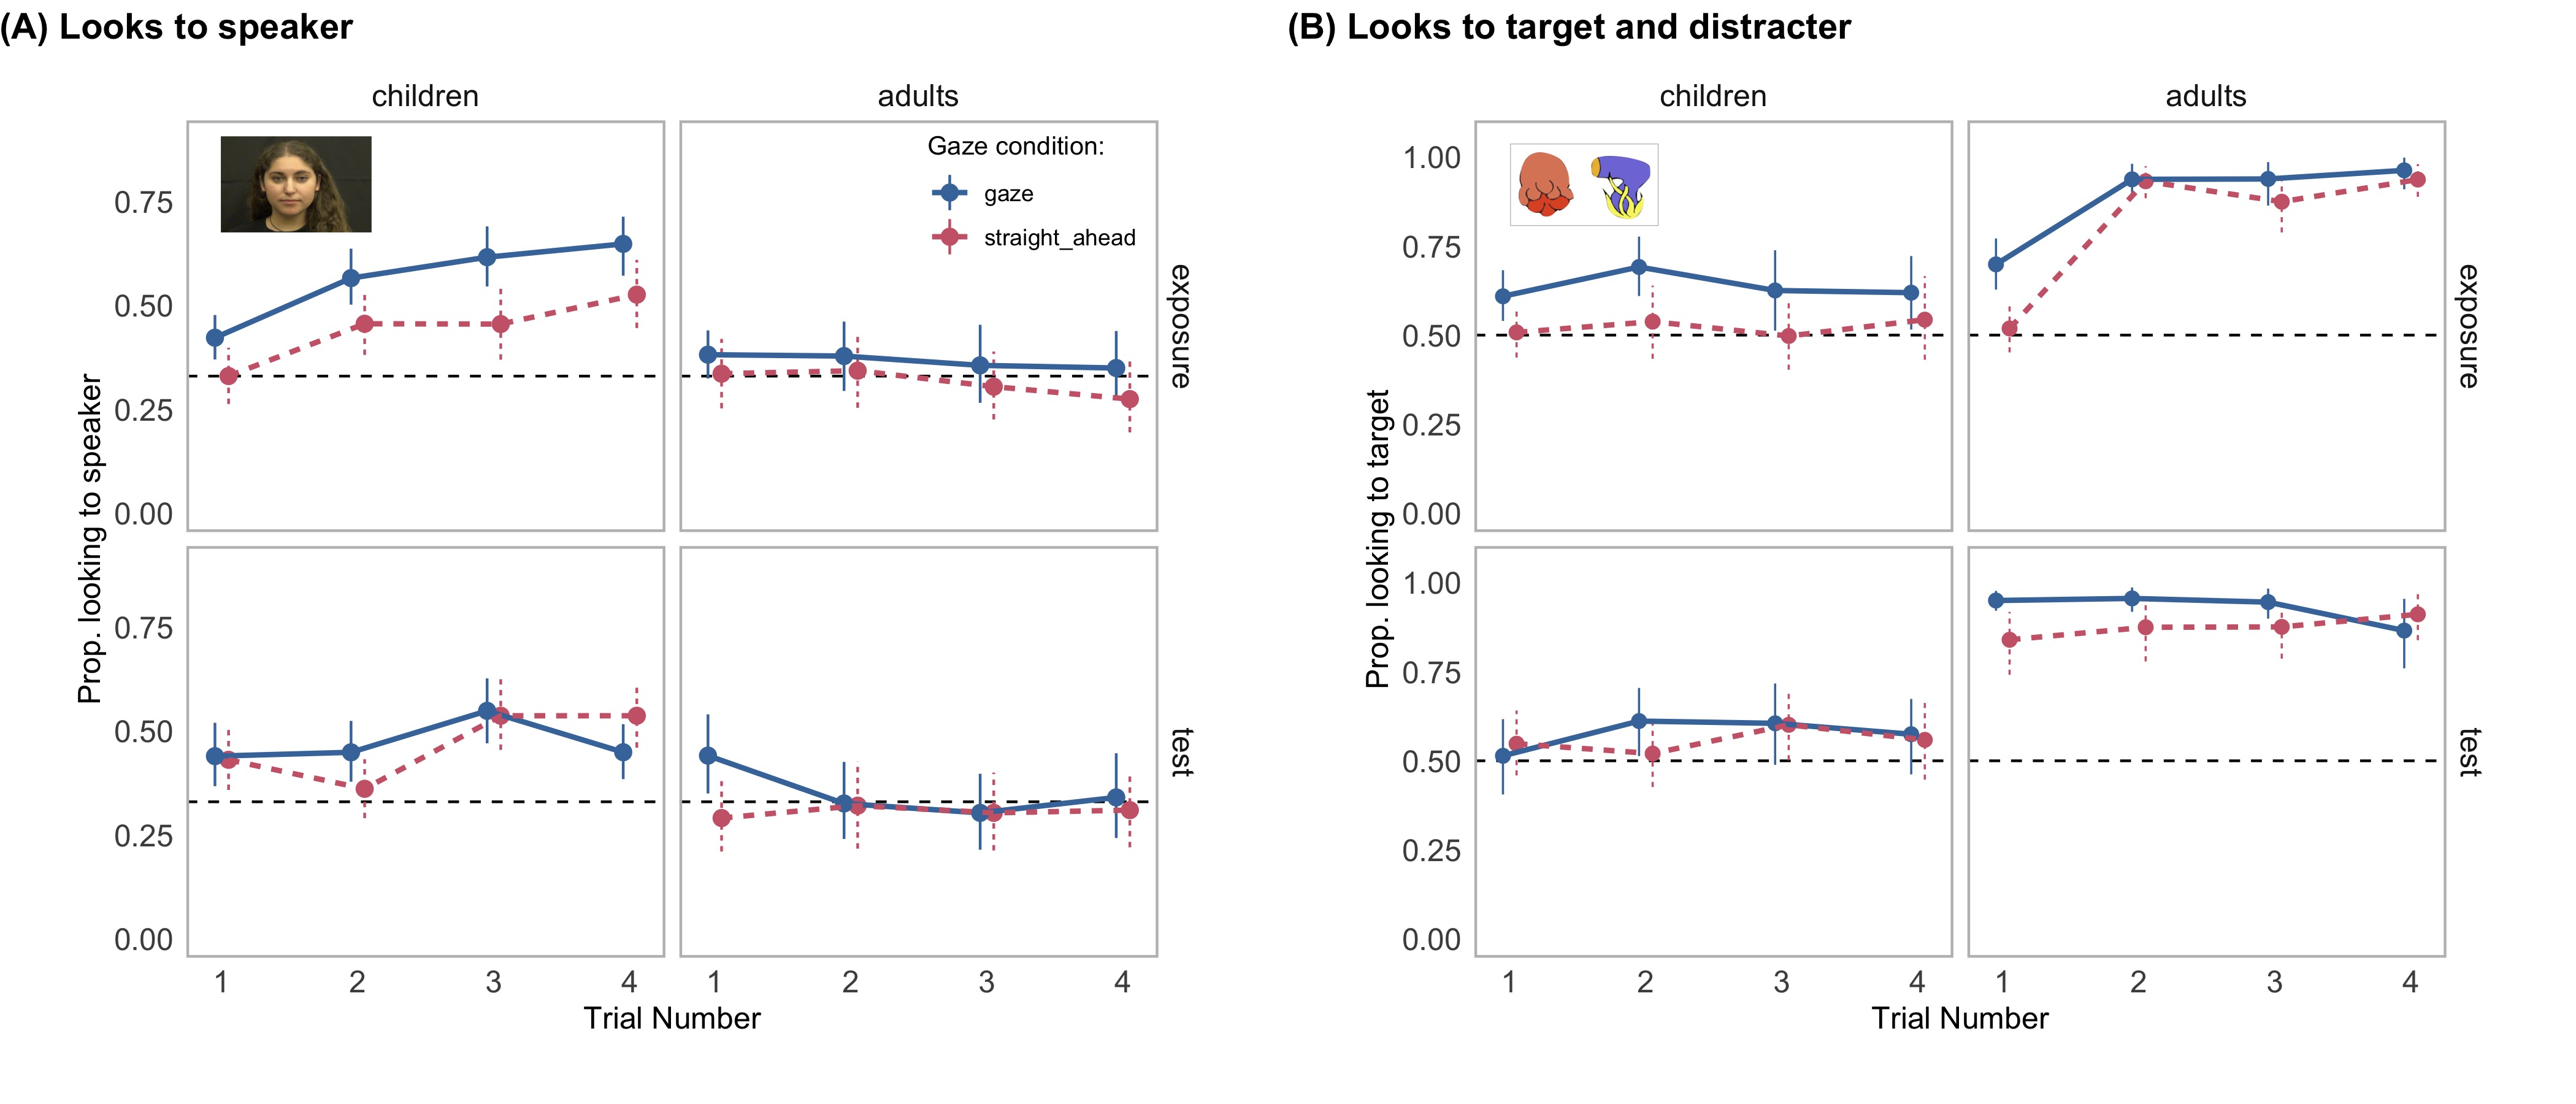
\includegraphics[width=0.95\linewidth]{/Users/kylemacdonald/Documents/Projects/SPEED-ACC-NOVEL/writing/figures/plots/speed_acc_novel_proplook} 

}

\caption[Panel A shows participants’ tendency to look at the speaker on exposure and test trials as a function of the trial number within a learning block]{Panel A shows participants’ tendency to look at the speaker on exposure and test trials as a function of the trial number within a learning block. The horizontal, dashed line represents the tendency to distribute attention equally across the three AOIs. Color indicates gaze condition and error bars represent 95\% credible intervals. Panel B shows the same information but for target and distracter looking across the learning block.}\label{fig:san-prop-looking-plot}
\end{figure*}
\end{CodeChunk}

\hypertarget{methods-1}{%
\subsection{Methods}\label{methods-1}}

\hypertarget{participants-1}{%
\subsubsection{Participants}\label{participants-1}}

Participants were native, monolingual English-learning children (\(n=\)
54; 30 F) and adults (\(n=\) 30; 20 F). All participants had no reported
history of developmental or language delay and normal vision. 6 adults
were run but not included because they were not native speakers of
English. 7 children participants were run but not included in the
analysis because the participant did not complete more than half of the
trials in the task.

\hypertarget{materials-1}{%
\subsubsection{Materials}\label{materials-1}}

\emph{Linguistic stimuli.} The video/audio stimuli were recorded in a
sound-proof room and featured two female speakers who used natural
child-directed speech and said one of two phrases: ``Hey! Can you find
the (novel word)'' or "Look! Where's the (novel word). The target words
were four pseudo-words: bosa, modi, toma, and pifo. The novel words
varied in length (shortest = 472.00 ms, longest = 736.00 ms) with an
average length of 606.31 ms.

\emph{Gaze manipulation}. The gaze manipulation was identical to
Experiment 1. The average length of gaze was 2.06 seconds with a range
from 1.74 to 2.67 seconds.

\emph{Visual stimuli.} The image set consisted of 28 colorful digitized
pictures of objects that were selected such that they would be
interesting to and that children would be unlikely to have already a
label associated with the objects. The side of the target picture was
counterbalanced across trials.

\hypertarget{procedure-1}{%
\subsubsection{Procedure}\label{procedure-1}}

The procedure was identical to Experiment 1. Participants watched a
series of ambiguous word learning events organized into pairs of one
exposure and one test trial. On each trial, participants saw a set of
two unfamiliar objects and heard one novel word. Each word occurred in a
block of four exposure-test pairs for a total of eight trials for each
novel word. On each trial within a learning block, one of the objects in
the set had consistently appeared on the previous trials (target
object), while the other object was a randomly generated novel object
that had not been shown in the experiment (distracter object).

\hypertarget{results-and-discussion-1}{%
\subsection{Results and Discussion}\label{results-and-discussion-1}}

\hypertarget{prediction-1-the-presence-of-gaze-increases-social-information-seeking.}{%
\subsubsection{Prediction 1: The presence of gaze increases social
information
seeking.}\label{prediction-1-the-presence-of-gaze-increases-social-information-seeking.}}

Our primary question of interest was whether listeners would seek a
post-nominal gaze cue when processing novel words. In line with our
prediction, we found evidence that both children and adults spent more
time fixating on a speaker when she provided a social cue to reference
provided a gaze cue (Fig. 3A \(\beta_{gaze}\) = 0.09 {[}0.16, 0.01{]}).
Moreover, both children (Gaze \(M_{rt}\) = 1,136.77 ms, No-gaze
\(M_{rt}\) = 878.37 ms) and adults (Gaze \(M_{rt}\) = 878.65 ms, No-gaze
\(M_{rt}\) = 726.99 ms) had slower RTs in the gaze condition
(\(\beta_{gaze}\) = -0.20, {[}-0.38, -0.01{]}), with no evidence of an
interaction between gaze condition and age group (\(\beta_{age*gaze}\) =
0.27, {[}0.11, 0.44{]}). This result provides key support for our
account that listeners would adapt their gaze to seek social information
when uncertainty over the incoming words was higher and supportive
visual information was more useful.

\hypertarget{prediction-2-the-tendency-to-fixate-on-a-speaker-decreases-faster-when-learning-from-gaze.}{%
\subsubsection{Prediction 2: The tendency to fixate on a speaker
decreases faster when learning from
gaze.}\label{prediction-2-the-tendency-to-fixate-on-a-speaker-decreases-faster-when-learning-from-gaze.}}

We predicted that RTs on exposure trials in the gaze condijtion would
decrease at a faster rate, reflecting a reduction in the need to seek
social information after being exposed to consistent word-object
pairings. In contrast to our prediction, however, we found a
developmental difference such that children, but not adults, were more
likely to \emph{increase} their tendency to fixate on the speaker over
the course of the learning block (Fig 3A, \(\beta_{age*tr.num}\) =
-0.07, {[}-0.11, -0.04{]}). This developmental difference suggests that
looking to a social partner may have been more useful for children who
were still trying to disambiguate the novel words; whereas adults showed
evidence of successful disambiguation after the second exposure trial
and could focus attention on the objects instead.

\hypertarget{prediction-3-faster-learning-of-novel-words-from-gaze-cues.}{%
\subsubsection{Prediction 3: Faster learning of novel words from gaze
cues.}\label{prediction-3-faster-learning-of-novel-words-from-gaze-cues.}}

Both children and adults showed evidence of learning the novel
word-object links by the end of the task, with the null value of 0.5
falling below the lower bound of the lowest credible interval for
children's target looking in the No-gaze context (95\% HDI {[}0.51,
0.60{]}). Looking to the target increased as listeners were exposed to
more word-object pairings during the task (\(\beta_{tr.num}\) = 0.16,
{[}0.09, 0.24{]}) and was higher when the novel word was accompanied by
a gaze cue (\(\beta_{gaze}\) = 0.14, {[}0.21, 0.06{]}). Moreover, both
children (Gaze \(M_{acc}\) = 0.64, No-gaze \(M_{acc}\) = 0.49) and
adults (Gaze \(M_{acc}\) = 0.89, No-gaze \(M_{acc}\) = 0.81) generated
more accurate first shifts on exposure trials in the gaze condition,
indicating they were following the gaze cue (\(\beta_{gaze}\) = -0.57,
{[}-1.13, 0.00{]}) and fixating less on the distracter object.

Visual inspection of the top row of Fig \ref{fig:san-prop-looking-plot}B
shows that on the first exposure trial, both adults and children used
the gaze cue to disambiguate reference, fixating more on the target in
the gaze condition. In contrast, adults target looking reached ceiling
for both the gaze and no-gaze conditions by trial number two, indicating
that they had successfully used co-occurrence information to learn the
words. Finally, on test trials, adults tended to look more to the target
object when learning from a gaze cue, only reaching similar levels of
accuracy in the no-gaze condition at the end of the learning block.
There was not strong evidence, however, that the gaze manipulation
influenced children's looking behavior on test trials when there was no
gaze cue present, with children showing comparable and relatively
low-levels of accuracy overall.

Contrary to our prediction, we did not see evidence that the gaze
manipulation led children or adults to generate more accurate first
shifts on test trials (\(\beta_{gaze}\) = -0.50, {[}-1.14, 0.14{]}) or a
faster increase in first shift accuracy over the course of learning
(\(\beta_{gaze*tr.num}\) = -0.30, {[}-0.74, 0.12{]}), with the null
value falling within each credible interval.

\hypertarget{general-discussion}{%
\section{General Discussion}\label{general-discussion}}

Does social information seeking change as a function of a speaker's
helpfulness and listeners' current task goals? Here, we pursued the idea
that listeners flexibly adapt their eye movements to gather social gaze
when it was useful. We found that children and adults did not
automatically delay their gaze shifts to seek a post-nominal gaze cue
while processing familiar words. Howeer, when processing novel words,
both children and adults fixated more on a speaker to seek a
post-nominal gaze cue. This delay resulted in more attention allocated
to the named object and less looking to the distracter object, an effect
that increased throughout the task for children. Moreover, adults, but
not children, showed evidence of stronger learning in the presence of
social gaze while both age groups were capable of learning the
word-object pairings from cross-situational statistics alone.

How should we characterize the effects of gaze on information seeking
and word learning in our task? Children selectively gathered social
information when they were uncertain about the meaning of a new word,
focusing attention on a single object. This pattern of behavior
generalized to trials without a gaze cue, showing how the effect of gaze
could accumulate over time. Finally, seeking social gaze increased the
rate of word learning for adults. This finding dovetails with other work
showing that the presence of social information changes information
processing (Wu, Gopnik, Richardson, \& Kirkham, 2011; Yoon, Johnson, \&
Csibra, 2008).

We did not find strong evidence that the effects of gaze generalized to
contexts without gaze for children in Experiment 2. Moreover, children
did not show strong learning of the novel word-object links overall.
Prior work has shown that 3-5 year-olds learn words better from an
extended, as opposed to brief, social cue to reference (Yurovsky, Wade,
\& Frank, 2013). Future work could increase the length of the gaze cue,
which was relatively short in these studies (\textasciitilde{}2 sec) or
could include a wider set of cues to reference such as pointing or
holding objects.

These results show that even young listeners are sensitive to the
informational tradeoffs in active information gathering. We found that
both children and adults' decisions to seek social information varied
depending on their uncertainty over word-object mappings. In the context
of processing novel, but not familiar words, listeners adapted their
gaze to seek a post-nominal social cue to reference. This change led to
increased visual attention on a single object and less attention
distributed across potential spurious word-object links. This approach
sheds light on how children might integrate their prior knowledge
accumulated via statistical information when deciding whether to seek
information from their interlocutors during real time language
processing.

\vspace{1em}

\fbox{\parbox[b][][c]{7.3cm}{\centering Data/code available at \url{https://bit.ly/2FgIbsW} \\ E1 preregistration at \url{https://osf.io/2q4gw/}\\ E2 preregistration at \url{https://osf.io/nfz85/}}}
\vspace{1em}

\hypertarget{acknowledgements}{%
\section{Acknowledgements}\label{acknowledgements}}

Thanks to Kayla Constandse, Tami Alade, and Hannah Slater for help with
data collection. This work was supported by an NSF GRFP to KM and a
Jacobs Foundation Fellowship to MCF.

\hypertarget{references}{%
\section{References}\label{references}}

\setlength{\parindent}{-0.1in} 
\setlength{\leftskip}{0.125in}

\noindent

\hypertarget{refs}{}
\leavevmode\hypertarget{ref-baldwin1993infants}{}%
Baldwin, D. A. (1993). Infants' ability to consult the speaker for clues
to word reference. \emph{Journal of Child Language}, \emph{20}(02),
395--418.

\leavevmode\hypertarget{ref-bloom2002children}{}%
Bloom, P. (2002). \emph{How children learn the meaning of words}. The
MIT Press.

\leavevmode\hypertarget{ref-burkner2017brms}{}%
Bürkner, P.-C. (2017). Brms: An r package for bayesian multilevel models
using stan. \emph{Journal of Statistical Software}, \emph{80}(1), 1--28.

\leavevmode\hypertarget{ref-estigarribia2007getting}{}%
Estigarribia, B., \& Clark, E. V. (2007). Getting and maintaining
attention in talk to young children. \emph{Journal of Child Language},
\emph{34}(4), 799--814.

\leavevmode\hypertarget{ref-fourtassiword2018}{}%
Fourtassi, A., \& Frank, M. C. (2017). Word identification under
multidomodal uncertainty. In \emph{Proceedings of the 39th annual
conference of the cognitive science society}.

\leavevmode\hypertarget{ref-gibson2013rational}{}%
Gibson, E., Bergen, L., \& Piantadosi, S. T. (2013). Rational
integration of noisy evidence and prior semantic expectations in
sentence interpretation. \emph{Proceedings of the National Academy of
Sciences}, 201216438.

\leavevmode\hypertarget{ref-hayhoe2005eye}{}%
Hayhoe, M., \& Ballard, D. (2005). Eye movements in natural behavior.
\emph{Trends in Cognitive Sciences}, \emph{9}(4), 188--194.

\leavevmode\hypertarget{ref-kelly2010two}{}%
Kelly, S. D., Özyürek, A., \& Maris, E. (2010). Two sides of the same
coin: Speech and gesture mutually interact to enhance comprehension.
\emph{Psychological Science}, \emph{21}(2), 260--267.

\leavevmode\hypertarget{ref-macdonald2018children}{}%
MacDonald, K., Marchman, V. A., Fernald, A., \& Frank, M. C. (2018).
Children flexibly seek visual information during signed and spoken
language comprehension.

\leavevmode\hypertarget{ref-maris2007nonparametric}{}%
Maris, E., \& Oostenveld, R. (2007). Nonparametric statistical testing
of eeg-and meg-data. \emph{Journal of Neuroscience Methods},
\emph{164}(1), 177--190.

\leavevmode\hypertarget{ref-smith2013visual}{}%
Smith, L. B., \& Yu, C. (2013). Visual attention is not enough:
Individual differences in statistical word-referent learning in infants.
\emph{Language Learning and Development}, \emph{9}(1), 25--49.

\leavevmode\hypertarget{ref-vigliocco2014language}{}%
Vigliocco, G., Perniss, P., \& Vinson, D. (2014). Language as a
multimodal phenomenon: Implications for language learning, processing
and evolution. The Royal Society.

\leavevmode\hypertarget{ref-wu2011infants}{}%
Wu, R., Gopnik, A., Richardson, D. C., \& Kirkham, N. Z. (2011). Infants
learn about objects from statistics and people. \emph{Developmental
Psychology}, \emph{47}(5), 1220.

\leavevmode\hypertarget{ref-yoon2008communication}{}%
Yoon, J. M., Johnson, M. H., \& Csibra, G. (2008). Communication-induced
memory biases in preverbal infants. \emph{Proceedings of the National
Academy of Sciences}, \emph{105}(36), 13690--13695.

\leavevmode\hypertarget{ref-yurovsky2017preschoolers}{}%
Yurovsky, D., Case, S., \& Frank, M. C. (2017). Preschoolers flexibly
adapt to linguistic input in a noisy channel. \emph{Psychological
Science}, \emph{28}(1), 132--140.

\leavevmode\hypertarget{ref-yurovsky2013online}{}%
Yurovsky, D., Wade, A., \& Frank, M. (2013). Online processing of speech
and social information in early word learning. In \emph{Proceedings of
the annual meeting of the cognitive science society} (Vol. 35).

\bibliographystyle{apacite}


\end{document}
